\subsection{Funkcionalnosti aplikacije}

\begin{figure}[H]
	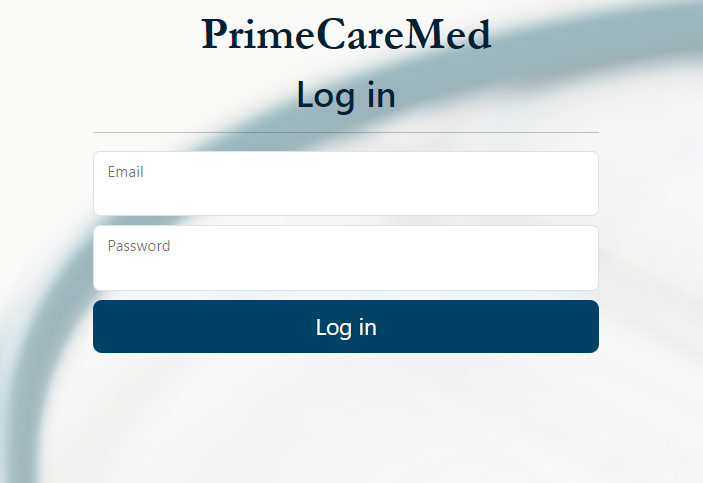
\includegraphics[width=1\linewidth,clip=]{assets/loginForma.png}
	\centering
	\caption{Login forma}
	\label{fig:loginForm}
\end{figure}

Na slici~\ref{fig:loginForm} prikazana je forma za prijavu korisnika dobivena pomoću Scaffold Identitya. Nakon uspješnog unosa korisničkog imena i lozinke, korisnik se autenticira u sustav ili mu se odbija pristup u slučaju krivo unesenih podataka. Uspješnom prijavom autenticirani korisnik ima pristup resursima aplikacije za koje njegova korisnička uloga ima postavljena autorizacijska prava. Korisnici s ulogom \texttt{Administrator} i \texttt{SysAdministrator} odmah nakon uspješne autentikacije preusmjeravaju se na glavni aplikacijski izbornik. Autenticirani korisnici s ulogom \texttt{Doctor} ili \texttt{Nurse} preusmjeravaju se na formu za odabir smjene te nemaju pravo korištenja aplikacije dok ne ispune taj međukorak. Provjera poveznice doktora, medicinske sestre i pripadajuće smjene implementirana je kolačićima.

\begin{figure}[H]
	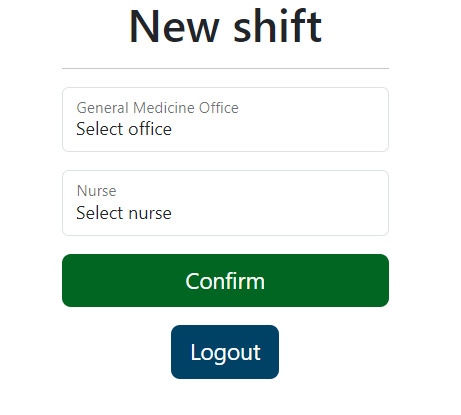
\includegraphics[width=0.6\linewidth,clip=]{assets/formaShift.png}
	\centering
	\caption{Forma za odabir smjene}
	\label{fig:shiftForm}
\end{figure}

Nakon prijave u sustav, korisnici s ulogom \texttt{Doctor} ili \texttt{Nurse} preusmjereni su na stranicu za odabir smjene. Ako je za trenutnog korisnika već odabrana smjena, bit će preusmjeren na glavni izbornik. Nakon odabrane smjene, podatci o novoj smjeni spremljeni su u kolačiće i korišteni za prikaz na izborniku što je vidljivo na slici~\ref{fig:newAppointment}.

\begin{figure}[H]
	
\includegraphics[width=1\linewidth,clip=]{assets/sysAdminIndex.png}
	\centering
	\caption{Početna stranica aplikacije}
	\label{fig:homePage}
\end{figure}

Na slici~\ref{fig:homePage} prikazana je početna stranica aplikacije s izbornikom s lijeve strane za korisnika s ulogom \texttt{SysAdministrator}. Broj izbora na spomenutom izborniku ovisi o ulozi korisnika.

\begin{figure}[H]
	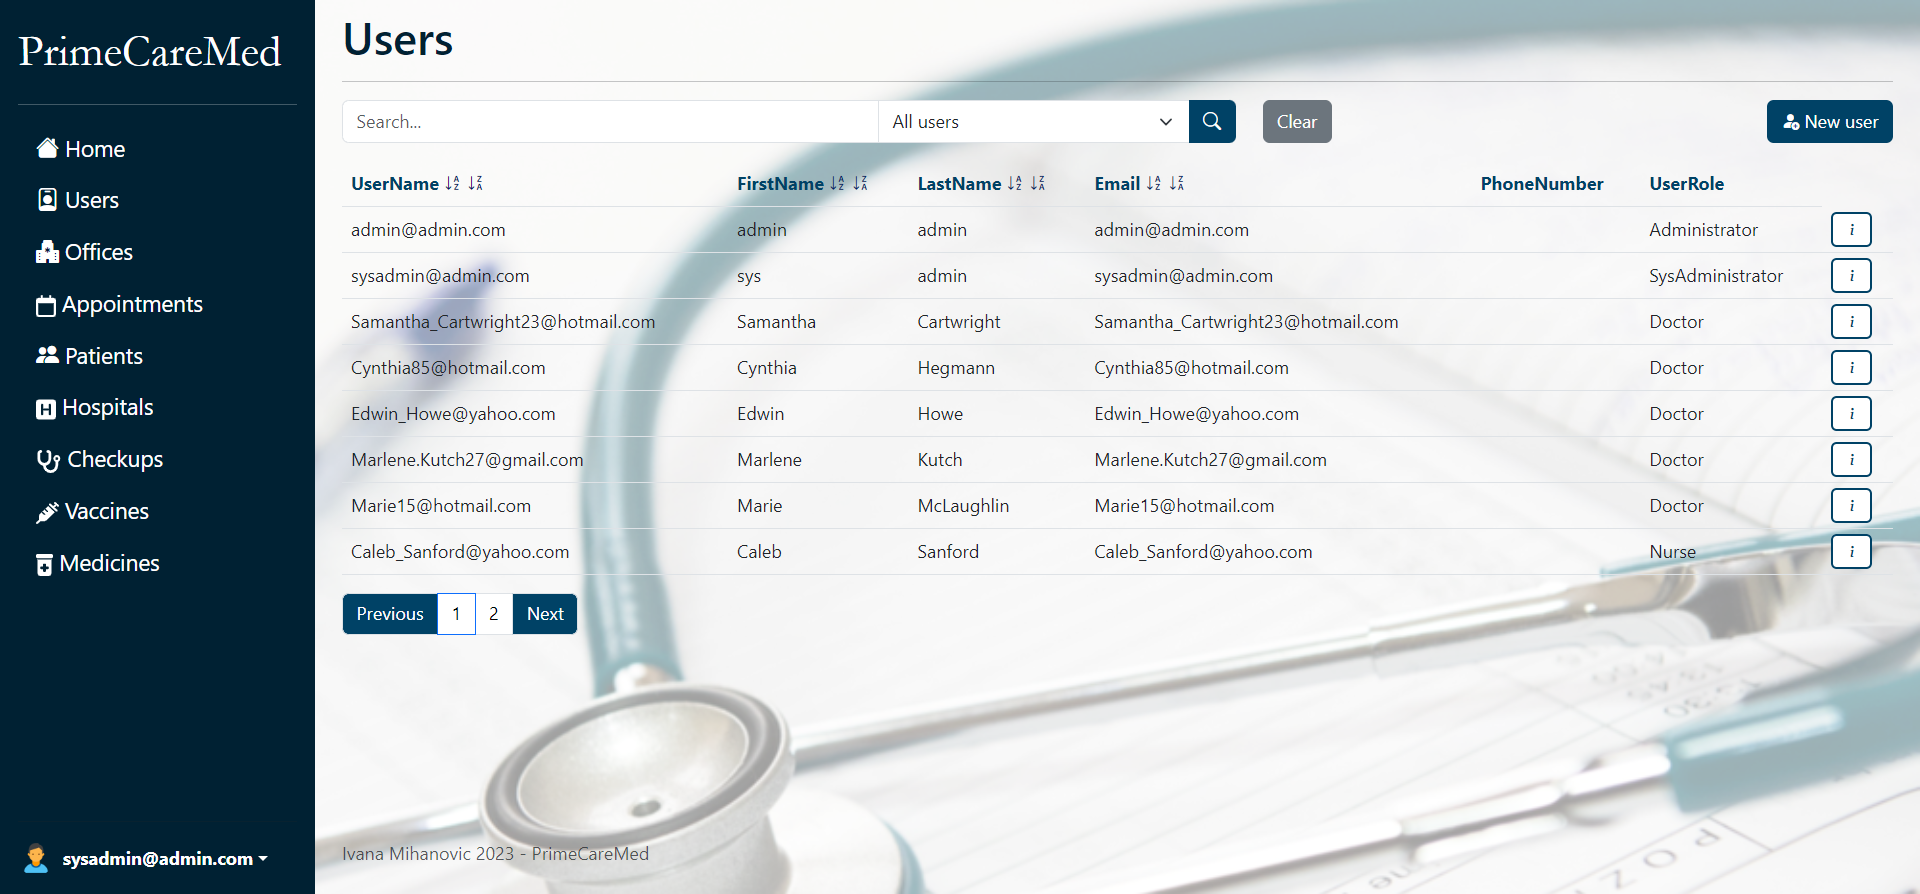
\includegraphics[width=1\linewidth,clip=]{assets/viewAllUsers.png}
	\centering
	\caption{Prikaz svih korisnika aplikacije}
	\label{fig:allUsers}
\end{figure}

Korisnicima s ulogom \texttt{Administrator} ili \texttt{SysAdministrator} omogućen je prikaz svih korisnika aplikacije. Na stranicu su implementirane mogućnosti pretrage, filtriranja i sortiranja zapisa. Za svakog korisnika postoji i botun s kojim je omogućeno uređivanje podataka i brisanje pacijenta iz sustava.

\begin{figure}[H]
	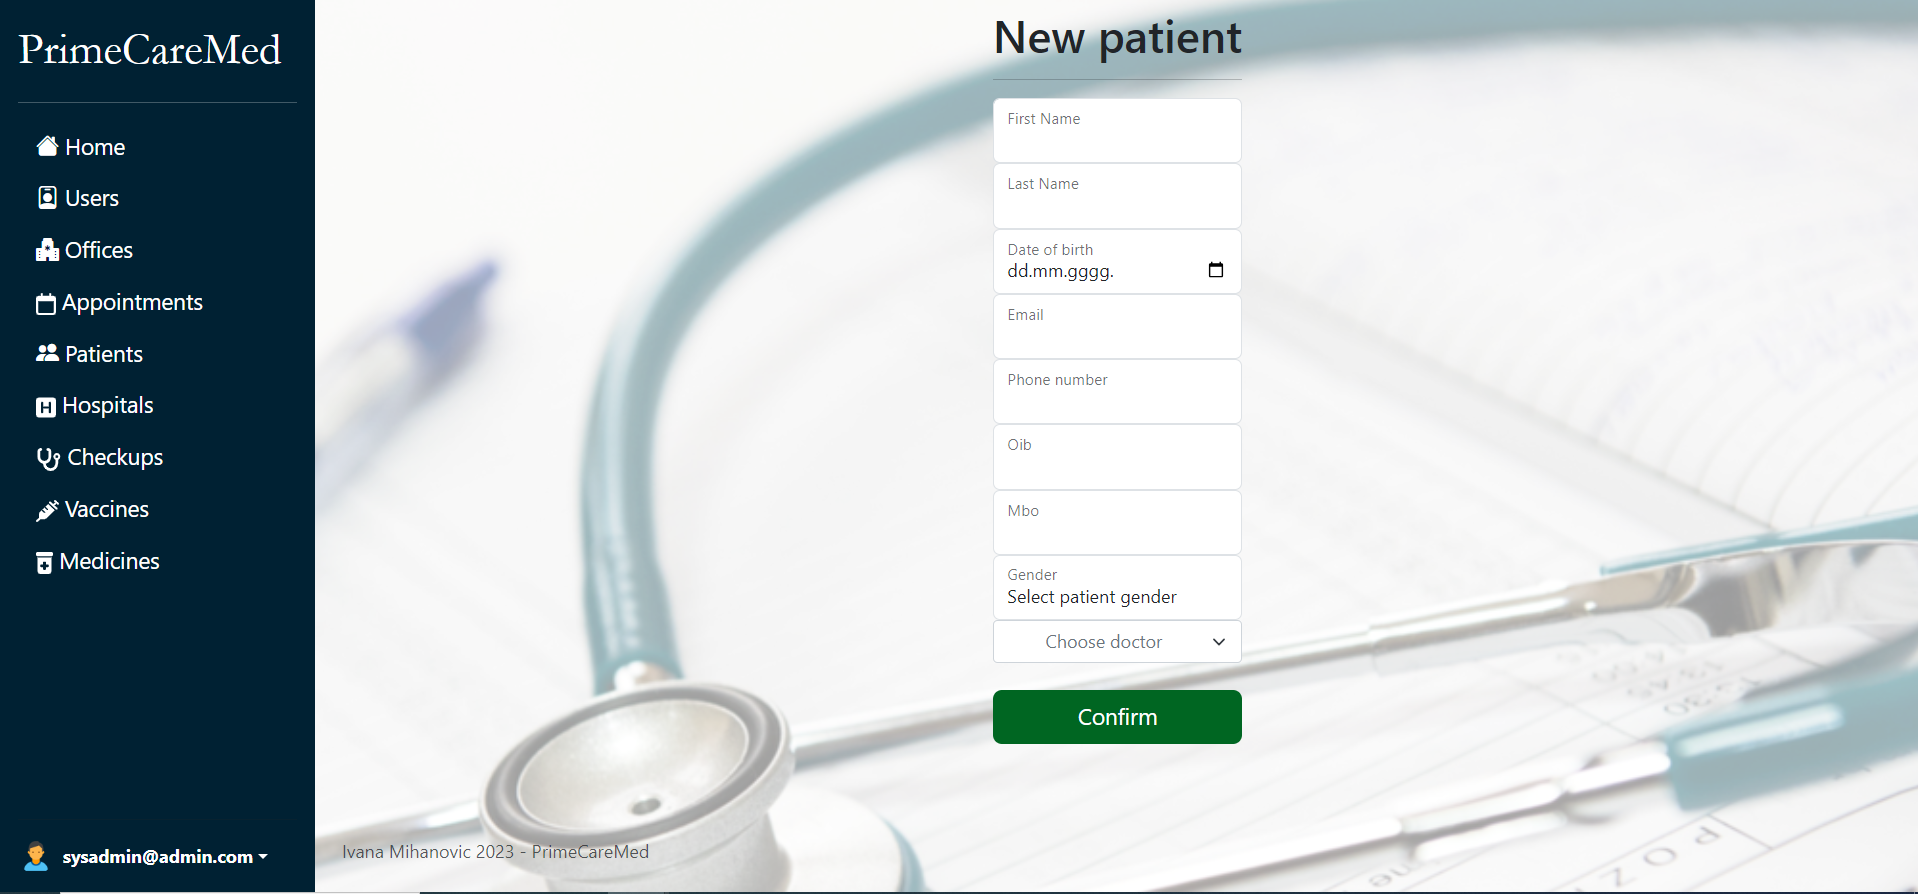
\includegraphics[width=1\linewidth,clip=]{assets/newPatient.png}
	\centering
	\caption{Unos novog pacijenta}
	\label{fig:newPatient}
\end{figure}

Slika~\ref{fig:newPatient} prikazuje formu za unos novog pacijenta u sustav. Prilikom kreiranja novog pacijenta u sustav, unose se svi potrebni podatci. Najvažniji podatci su \texttt{OIB} i \texttt{MBO} koji jedinstveno identificiraju pacijenta. \texttt{OIB} i \texttt{MBO} su tekstualna \textit{string} polja kako bi se omogućilo pravilno spremanje vrijednosti u bazu podataka ako polje počinje s nulom. U svrhu zaštite integriteta podataka ograničen je unos samo znamenki te se \texttt{OIB} sastoji od jedanaest, a \texttt{MBO} od devet znamenki. Sva polja za unos su obavezna osim odabira određenog doktora. 

\begin{figure}[H]
	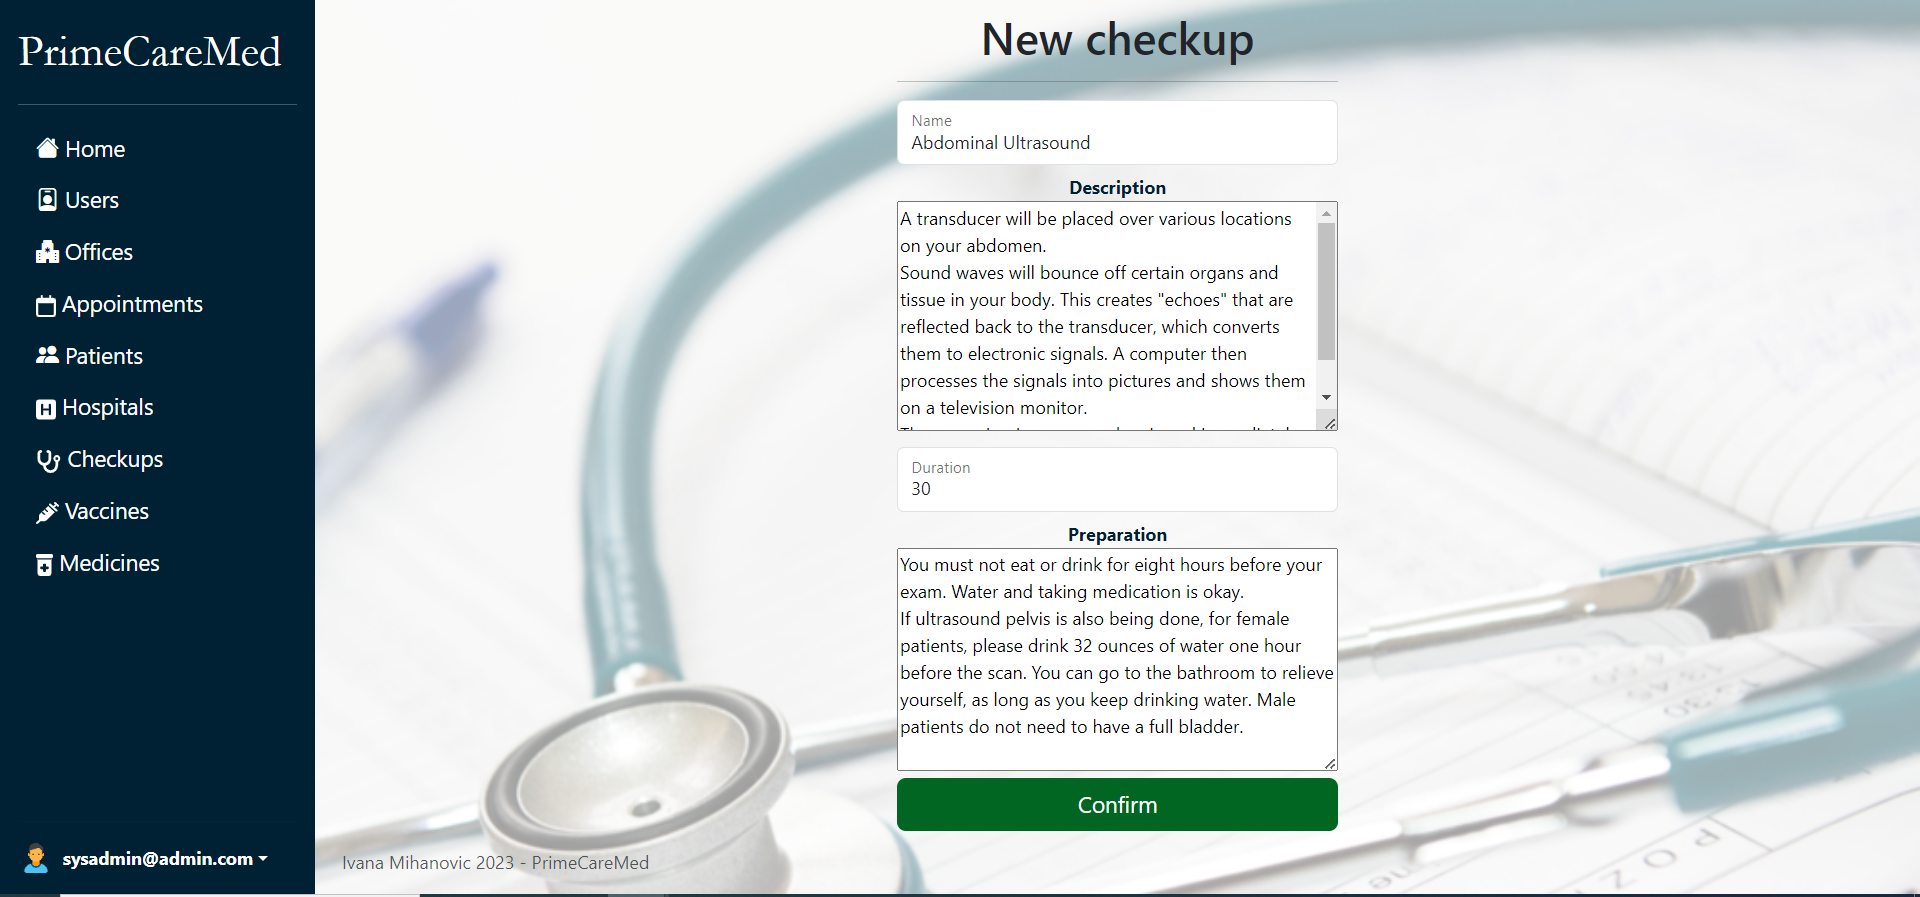
\includegraphics[width=1\linewidth,clip=]{assets/newCheckup.png}
	\centering
	\caption{Forma za unos novog \texttt{Checkup} entiteta}
	\label{fig:newCheckup}
\end{figure}

Na slici~\ref{fig:newCheckup} prikazana je forma za unos. Za navedenu stranicu prikazani su ispisi~\ref{subsubsec:.cshtml} za \texttt{.cshtml} i ispis~\ref{subsubsec:.cshtml.cs} za \texttt{.cshtml.cs} datoteke. Nakon spremanja, korisnik je preusmjeren na stranicu prikazanu na slici~\ref{fig:allCheckups}.

\begin{figure}[H]
	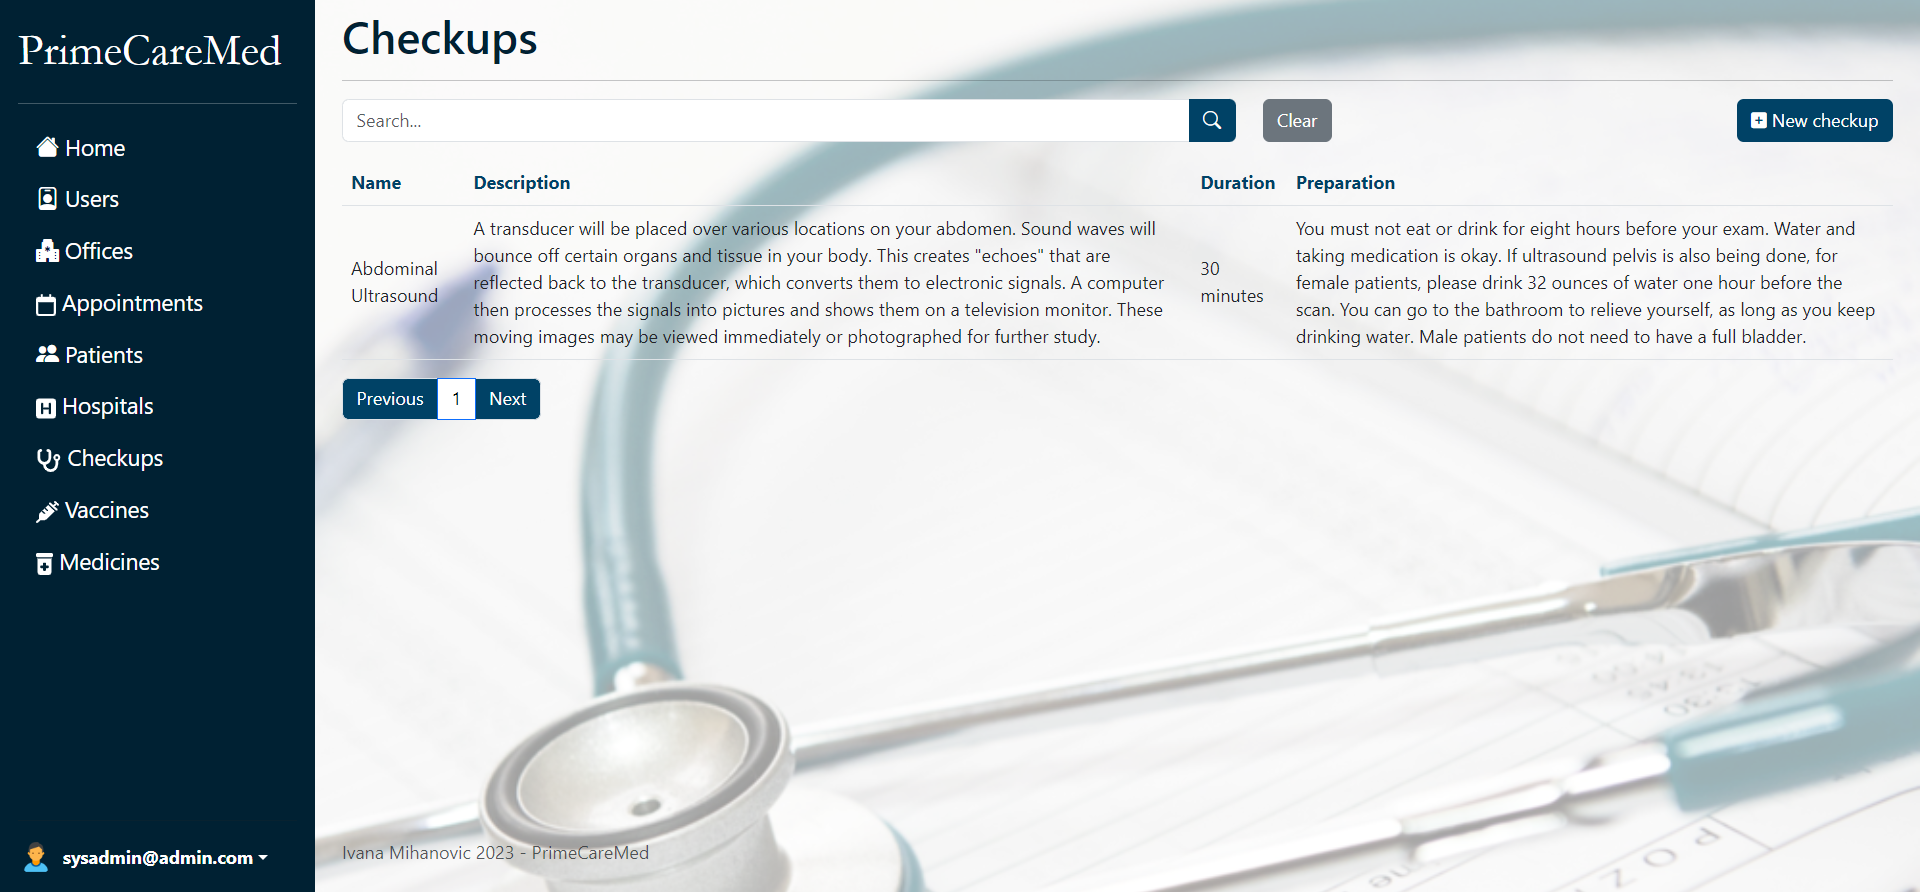
\includegraphics[width=1\linewidth,clip=]{assets/allCheckups.png}
	\centering
	\caption{Prikaz svih elemenata entiteta \texttt{Checkup}}
	\label{fig:allCheckups}
\end{figure}

\begin{figure}[H]
	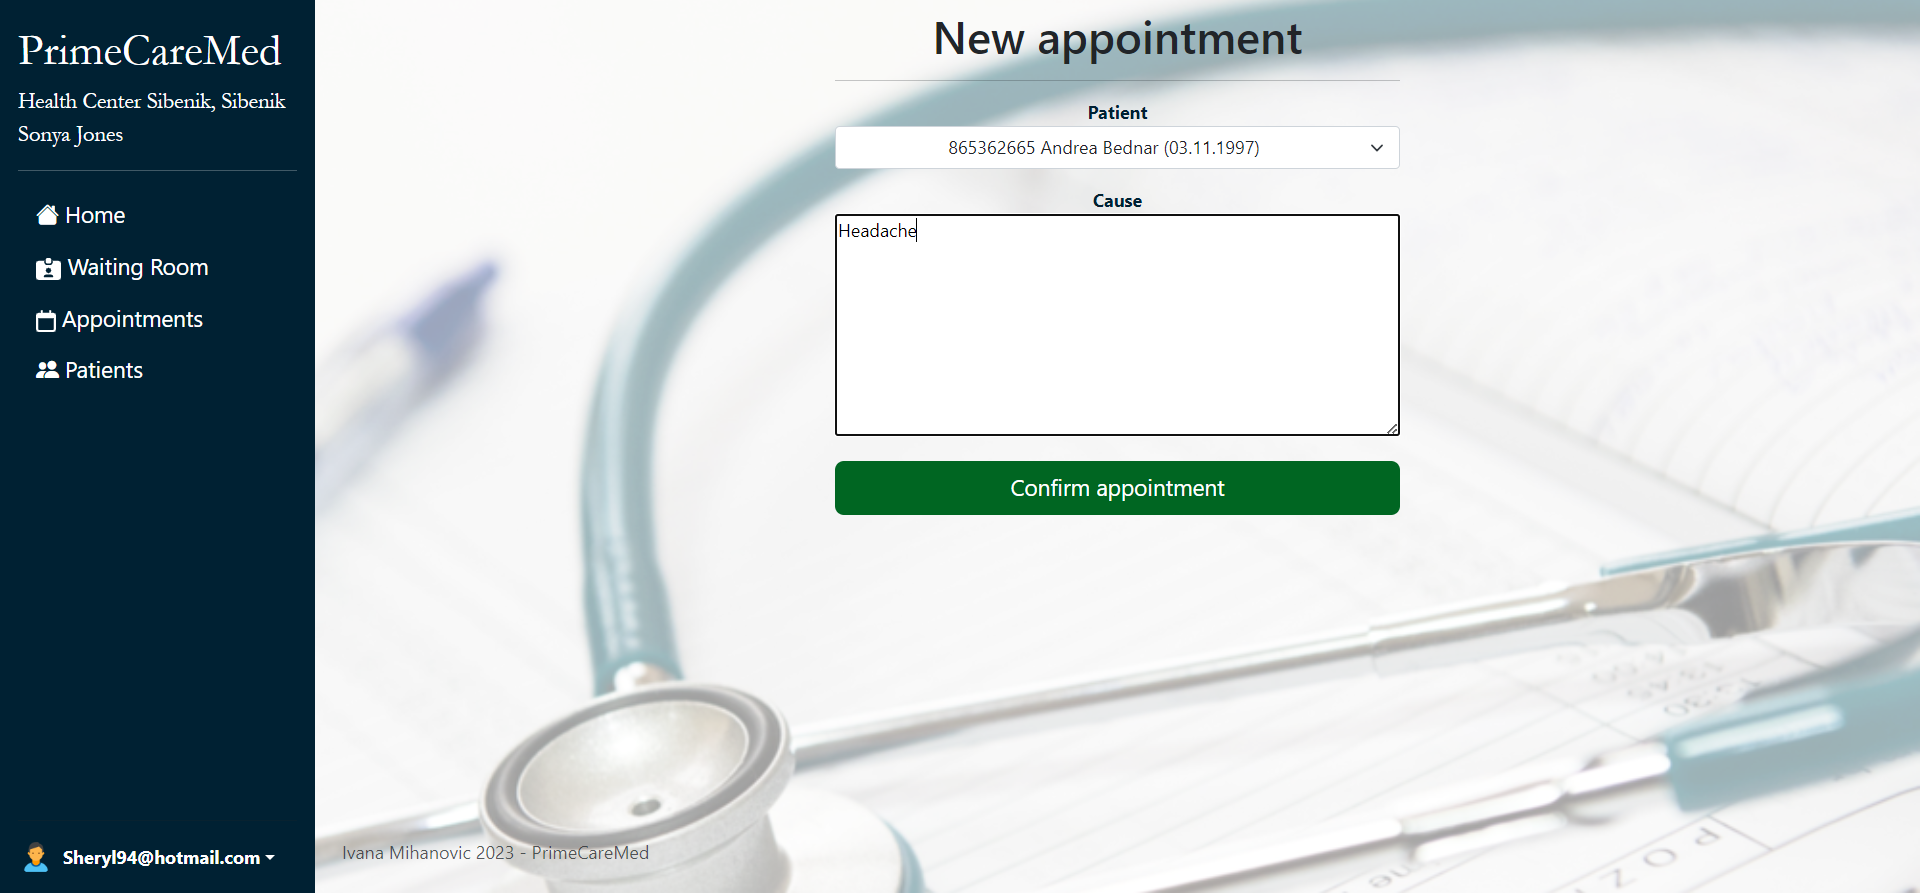
\includegraphics[width=1\linewidth,clip=]{assets/newAppointment.png}
	\centering
	\caption{Unos novog pregleda u čekaonicu}
	\label{fig:newAppointment}
\end{figure}

Na slici~\ref{fig:newAppointment} prikazan je unos novog pregleda u čekaonicu za koji se odabire pacijent koristeći \texttt{Select2} padajući izbornik i unosi se razlog dolaska. Nakon unosa, korisnik je preusmjeren na stranicu koja predstavlja čekaonicu \texttt{WaitingRoom} ili na prikaz svih pregleda ovisno o ulozi.

\begin{figure}[H]
	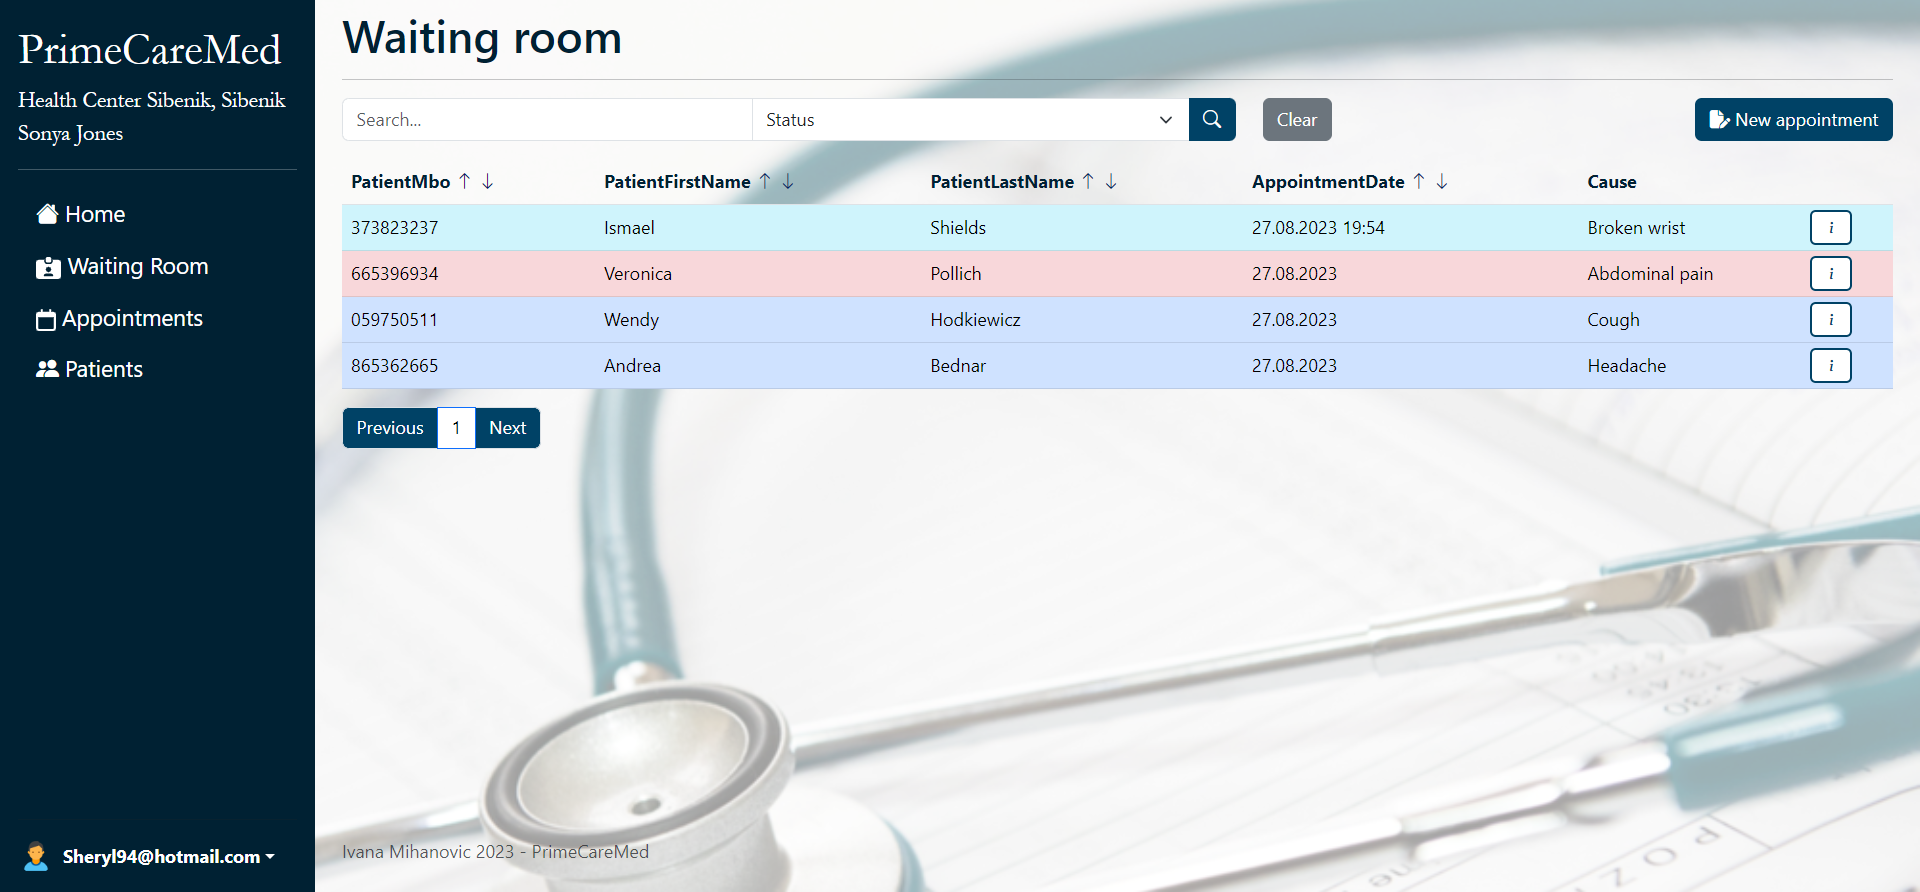
\includegraphics[width=1\linewidth,clip=]{assets/waitingRoom.png}
	\centering
	\caption{Čekaonica}
	\label{fig:waitingRoom}
\end{figure}

Slika~\ref{fig:waitingRoom} prikazuje čekaonicu za korisnike s ulogama \texttt{Doctor} i \texttt{Nurse}. Pojedini status pregleda, označen je zasebnom bojom.

\begin{figure}[H]
	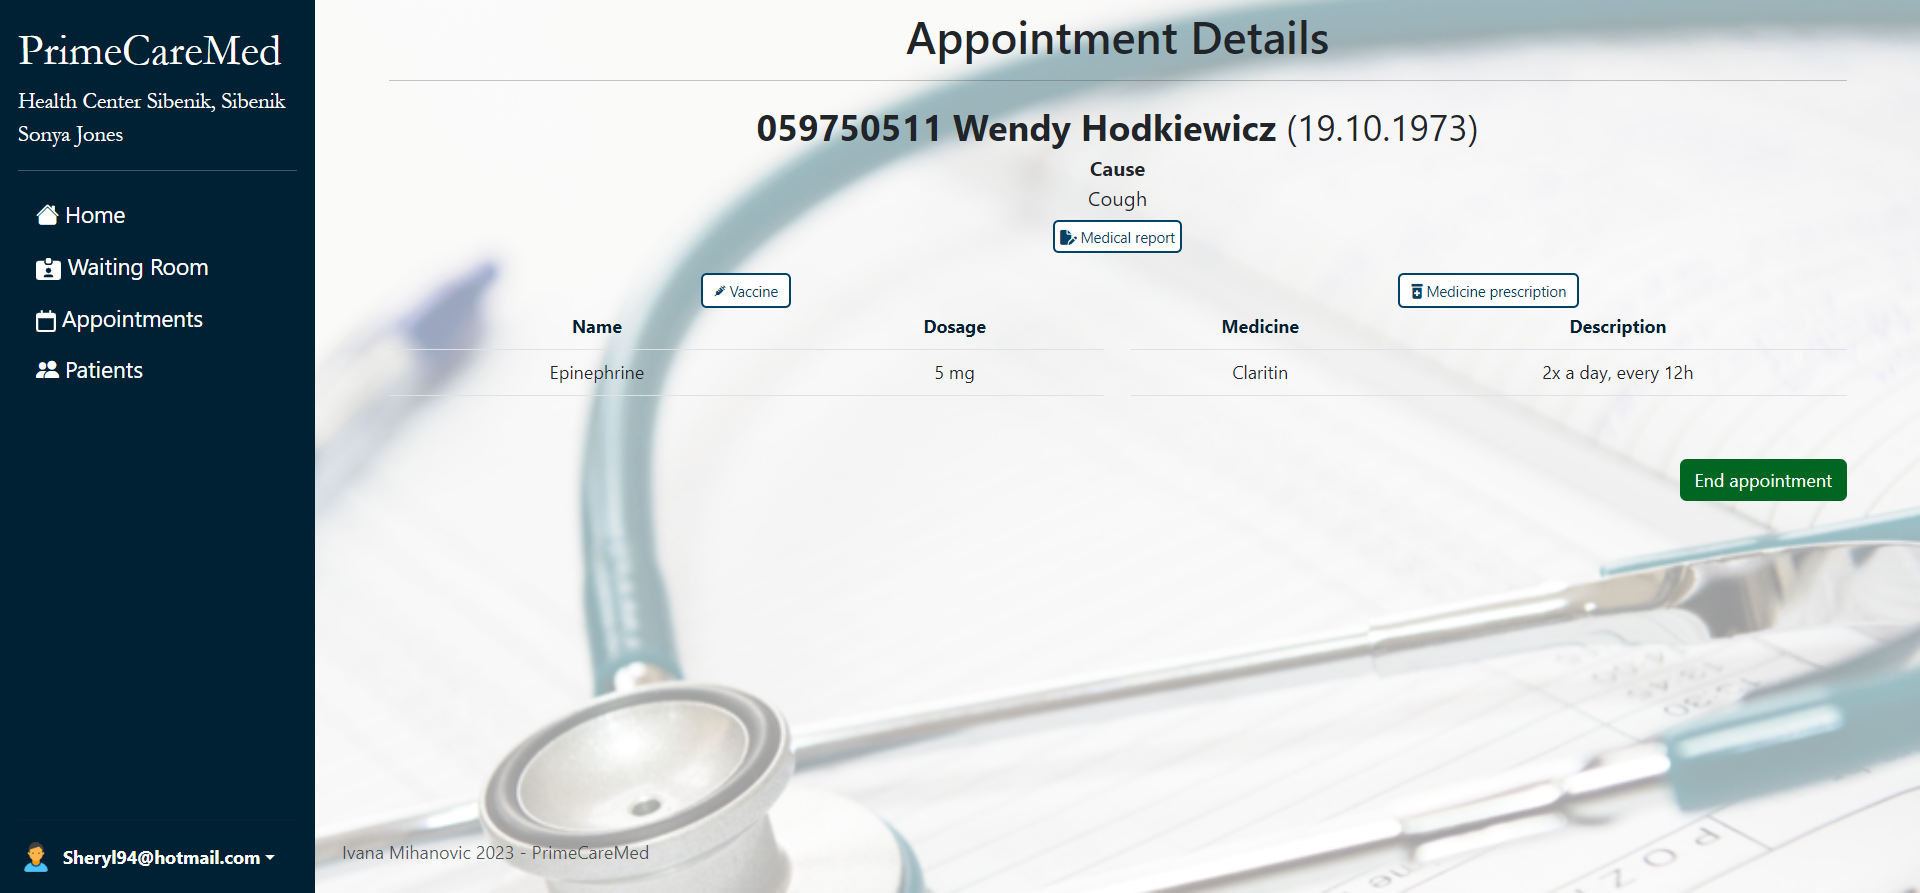
\includegraphics[width=1\linewidth,clip=]{assets/appointmentDetails.png}
	\centering
	\caption{Detalji pregleda}
	\label{fig:appointmentDetails}
\end{figure}

Pritiskom na botun za detalje pregleda, otvara se stranica prikazana na slici~\ref{fig:appointmentDetails} na kojoj je omogućen unos novih recepata za lijek, cjepiva i izvješća. Pritiskom na botun \texttt{End appointment}, status pregleda mijenja se na \texttt{Done} i tada su izmjene dostupne samo korisniku s ulogom \texttt{SysAdministrator}.

Na slikama~\ref{fig:newCheckupAppointment}, ~\ref{fig:dateCheckupAppointment} i~\ref{fig:timeCheckupAppointment} prikazan je postupak narudžbe pacijenta na pregled u bolnici.

\begin{figure}[H]
	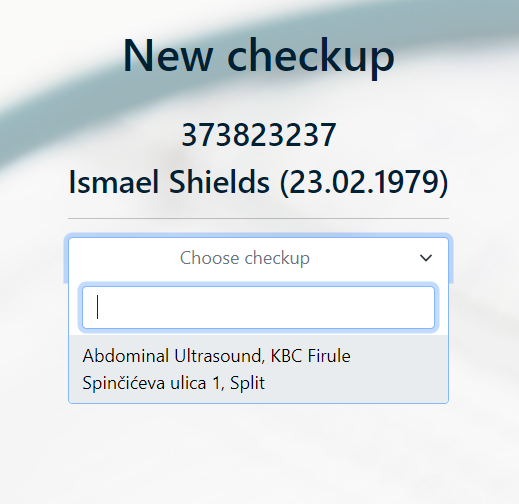
\includegraphics[width=0.6\linewidth,clip=]{assets/newCheckupAppointment.png}
	\centering
	\caption{Odabir pregleda}
	\label{fig:newCheckupAppointment}
\end{figure}

Na slici~\ref{fig:newCheckupAppointment} prikazan je početak narudžbe pacijenta na pregled u kojem liječnik odabire pregled pomoću \texttt{Select2} padajućeg izbornika.

\begin{figure}[H]
	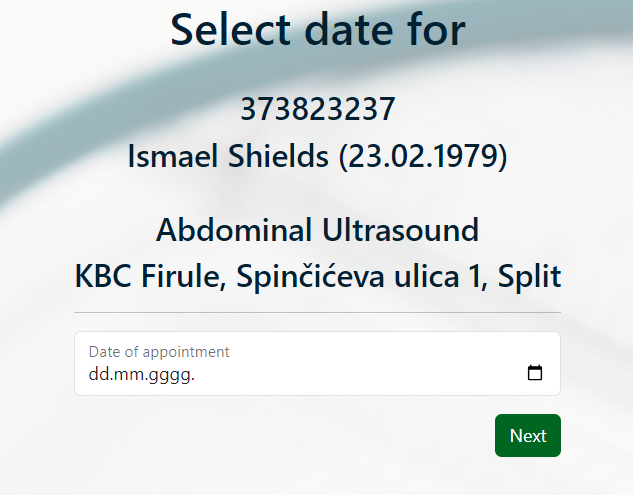
\includegraphics[width=0.6\linewidth,clip=]{assets/dateCheckupAppointment.png}
	\centering
	\caption{Odabir datuma pregleda}
	\label{fig:dateCheckupAppointment}
\end{figure}

Nakon odabira pregleda, liječnik odabire datum pregleda te je preusmjeren na stranicu prikazanu na slici~\ref{fig:timeCheckupAppointment} za odabir termina pregleda.

\begin{figure}[H]
	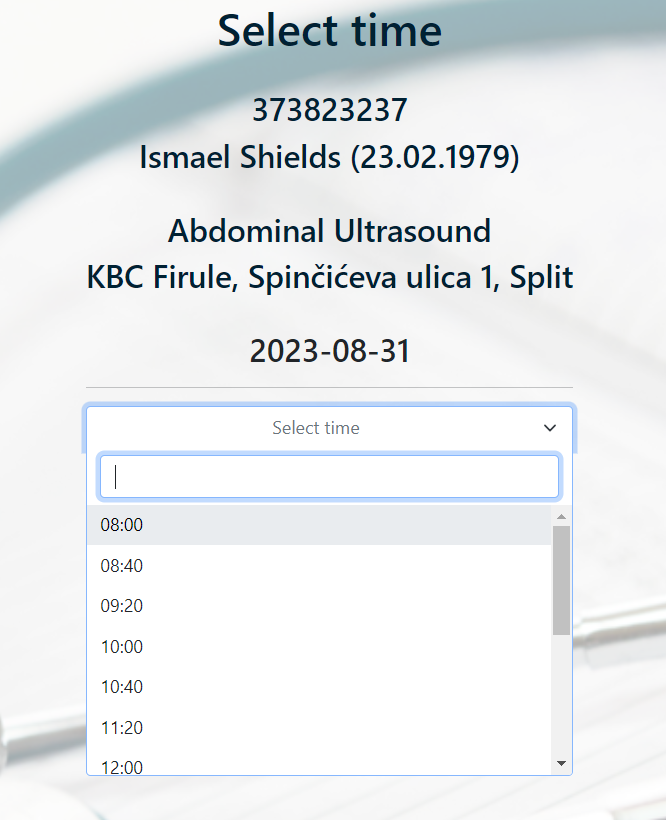
\includegraphics[width=0.6\linewidth,clip=]{assets/timeCheckupAppointment.png}
	\centering
	\caption{Odabir termina pregleda}
	\label{fig:timeCheckupAppointment}
\end{figure}

Prikazani su samo dostupni termini pregleda koji su generirani za pojedini pregled na temelju njegovog trajanja. Za svaki termin, moguće je napraviti četiri narudžbe. Kada su četiri narudžbe za isti pregled u isto vrijeme kreirane sa statusom \texttt{Active}, ne prikazuje se navedeni termin u padajućem izborniku.